%% For the SIAM style do the following:
%% 1. Change the document class
%% 2. Turn off all lines in preamble excpet macros, title and author 
%% 3. Turn on section about keywords, ACM and pagestyle
%% 4. Change bibliography style
%% 5. In "The effective order of RK methods" section turn on order conditions table
%% 6. In  "Optimal ESSPRK methods" section turn on the two tables for ESSPRK(4,4,2) and ESSPRK(4,4,3)
%% Required files for SIAM class: siamltex.cls, siamltex.sty, siam10.clo, subeqn.clo, siam.bst
%% available from http://www.siam.org/journals/auth-info.php 

\documentclass[10pt,a4paper,oneside]{article}
%\documentclass[final]{siamltex}  % SIAM class: use [final] to view lines that extend past the margin

%%%%%%%%%%%%%%%%%%%%%%%%%%%%%% Preamble %%%%%%%%%%%%%%%%%%%%%%%%%%%%%%  

%%% Turn off for SIAM style %%%
%%%%%%%%%%%%%%%%%%%%%%%
\usepackage{amsthm}
\usepackage[font=normalsize,position=top]{caption}
\captionsetup[subfloat]{position=bottom}
\setlength{\textwidth}{160mm}   
\setlength{\textheight}{220mm}
\setlength{\oddsidemargin}{0mm} 
\setlength{\evensidemargin}{-5mm}
\setlength{\topmargin}{0mm}
\setlength{\marginparwidth}{35mm}
\newcommand{\colintodo}[1]{\todo[color=orange!20]{\textbf{C:} #1}}
\newcommand{\davidtodo}[1]{\todo[color=cyan!20]{\textbf{D:} #1}}
\newcommand{\yiannistodo}[1]{\todo[color=green!20]{\textbf{Y:} #1}}
\newcommand{\colincomment}[1]{\textcolor{blue}{\\\textbf{\footnotesize #1}\\}}
\newcommand{\davidcomment}[1]{\textcolor{red}{\\\textbf{\footnotesize #1}\\}}
\newcommand{\yianniscomment}[1]{\textcolor{OliveGreen}{\\\textbf{\footnotesize #1}\\}}
\newtheorem{theorem}{Theorem}[section]
\newtheorem{definition}[theorem]{Definition}
\newtheorem{example}[theorem]{Example}
\newtheorem{lemma}[theorem]{Lemma}
\newtheorem{proposition}[theorem]{Proposition}
\newtheorem{corollary}[theorem]{Corollary}
%%%%%%%%%%%%%%%%%%%%%%%

%%% packages %%%
%\usepackage{enumerate,cite}
%\usepackage{caption} % [font=small,format=plain,labelfont=bf,up,textfont=it,up]
%\usepackage{verbatim}
%\usepackage{rotating}
%\usepackage{slashbox}
%\usepackage{xkeyval}
%\usepackage[normalem]{ulem}
%\usepackage[toc,page]{appendix}
%\usepackage{diagrams}
%\usepackage{nomencl}
%\usepackage{cm-super}
%\usepackage{ifthen}
%\usepackage{maplestd2e}
%\usepackage[numbered]{mcode}
%\usepackage{epsfig}
%\usepackage{calc}
%\usepackage{pbox}

%%% Page layout %%%
%\setlength{\parindent}{5mm}
%\setlength{\footskip}{20mm}
%\setlength\footnotesep{2mm}

%%% Page style %%%
%\pagestyle{plain}

%%% Renew commands %%%
%\renewcommand{\newline}{\vspace{10pt}}
%\renewcommand{\comment}[1]{\textcolor{gray}{\\#1\\}}
%\renewcommand{\indent}{\hspace{15pt}}
%\newcolumntype{M}[1]{>{\vspace{0.25pt}\centering\hspace{0pt}\vspace{0.25pt}}m{#1}}

%%% Miscellaneous %%%
% \numberwithin{theorem}{section}
% \numberwithin{equation}{section}
% \numberwithin{table}{section}
% \numberwithin{figure}{section}
%\numberwithin{theorem}{section}
%\numberwithin{equation}{section}
%\numberwithin{definition}{section}
%\numberwithin{example}{section}
%\setcounter{secnumdepth}{3}
%\setcounter{tocdepth}{3}
%\setcounter{table}{0}
%\baselineskip=18pt plus1pt
%\makenomenclature

%%% Supporting macros %%%
%%% packages %%%
\usepackage{amsmath,amssymb,amsfonts}
\usepackage[usenames,dvipsnames]{color}
\usepackage[dvips]{graphicx} % [pdftex]
\usepackage{pstricks,pst-node,pst-tree}
\usepackage{bm}
\usepackage{multirow}
\usepackage{multicol}
\usepackage{url}
\usepackage{array}
\usepackage{arydshln}
\usepackage[caption=false]{subfig}
\usepackage{booktabs}
\usepackage{accents}
\definecolor{lightgray}{gray}{0.5}
\definecolor{darkred}{rgb}{.6,0,0}
\definecolor{darkblue}{rgb}{0,0,0.5}
\usepackage[colorlinks=true,citecolor=darkblue,urlcolor=darkblue,linkcolor=darkred]{hyperref}
\usepackage[textsize=footnotesize]{todonotes}

%%% New commands %%%
\newcommand{\sspcoef}{\mathcal{C}}
\newcommand{\ceff}{\sspcoef_{\textnormal{eff}}}
\newcommand{\clin}{\sspcoef^{\textnormal{lin}}_{s,q}}
\newcommand{\pd}[2]{\frac{\partial{#1}}{\partial{#2}}}
\newcommand{\pdseconda}[2]{\frac{\partial^2{#1}}{\partial{{#2}^2}}}
\newcommand{\pdsecondb}[3]{\frac{\partial^2{#1}}{\partial{#2}\partial{#3}}}
\newcommand{\Dt}{\Delta t}
\newcommand{\DtFE}{\Delta t_{\textnormal{FE}}}
\newcommand{\equival}[1]{\mbox{{\large $\underaccent{\hspace{8pt}#1}{\simeq } \,$}}}
\newcommand{\rowscell}[2]{\parbox{21pt}{\centering #1 \\ #2}}
\newcommand{\treecell}[2]{\parbox{26pt}{\centering #1 \\\vspace{3pt} #2}}
\newcommand{\nline}{\tabularnewline\noalign{\vskip 2pt}}
\newcommand{\mydashrule}{%
  \noalign{\vskip 4pt}%
  \hdashline[2pt/3pt]%
  \noalign{\vskip 4pt}}
\newcommand{\mymidrule}{\midrule\noalign{\vskip 1.5pt}}
\newcolumntype{M}[1]{>{\vspace{0.25pt}\hspace{0pt}\vspace{0.25pt}}m{#1}}
\newcolumntype{L}[1]{>{\vspace{0.25pt}\hspace{-2.0pt}\vspace{0.25pt}}m{#1}}

%%% New theorems %%%
\newtheorem{remark}[theorem]{Remark}
\numberwithin{theorem}{section}
\numberwithin{equation}{section}
\numberwithin{table}{section}
\numberwithin{figure}{section}
 % additional macros
%%% Commands for drawing trees   %%%

% small trees
\newenvironment{smalltrees}{
	\psset{treesep=1.5ex,levelsep=1.2ex,treemode=U,showbbox=false}
	\renewcommand\psedge{\ncline[linewidth=0.6pt]}
	\renewcommand{\Ts}{\Tdot[dotstyle=*,dotscale=0.7]}
}

% large trees
\newenvironment{largetrees}{
    \psset{treesep=3ex,levelsep=3ex,treemode=U,showbbox=false}
    \renewcommand\psedge{\ncline[linewidth=1.0pt]}
    \renewcommand{\Ts}{\Tdot[dotstyle=*,dotscale=1.1]}
}

% medium trees
\psset{treesep=1.8ex,levelsep=1.8ex,treemode=U,showbbox=false}
\renewcommand\psedge{\ncline[linewidth=0.7pt]}
\newcommand{\Ts}{\Tdot[dotstyle=*,dotscale=0.9]}
\newcommand{\tree}[1]{
\ifthenelse{\equal{#1}{1}}{\raisebox{0.5ex}{{\pstree{\Ts}{}}}}{}%
\ifthenelse{\equal{#1}{2}}{\raisebox{0.0ex}{{\pstree{\Ts}{\Tn\Ts}}}}{}%
\ifthenelse{\equal{#1}{3}}{\raisebox{0.0ex}{{\pstree{\Ts}{\Ts\Ts}}}}{}%
\ifthenelse{\equal{#1}{4}}{\raisebox{-0.5ex}{{\pstree{\Ts}{\Tn\pstree{\Ts}{\Ts\Tn}}}}}{}%
\ifthenelse{\equal{#1}{5}}{\raisebox{0.0ex}{{\pstree{\Ts}{\Ts\Ts\Ts}}}}{}%
\ifthenelse{\equal{#1}{6}}{\raisebox{-0.5ex}{{\pstree{\Ts}{\Ts\pstree{\Ts}{\Ts\Tn}}}}}{}%
\ifthenelse{\equal{#1}{7}}{\raisebox{-0.5ex}{{\pstree{\Ts}{\Tn\pstree{\Ts}{\Ts\Ts}}}}}{}%
\ifthenelse{\equal{#1}{8}}{\raisebox{-0.7ex}{{\pstree{\Ts}{\Tn\pstree{\Ts}{\pstree{\Ts}{\Tn\Ts}\Tn}}}}}{}%
\ifthenelse{\equal{#1}{9}}{\raisebox{0.0ex}{{\pstree{\Ts}{\Ts\Ts\Ts\Ts}}}}{}%
\ifthenelse{\equal{#1}{10}}{\raisebox{-0.3ex}{{\pstree{\Ts}{\Ts\Ts\pstree{\Ts}{\Ts\Tn}}}}}{}%
\ifthenelse{\equal{#1}{11}}{\raisebox{-0.5ex}{{\pstree{\Ts}{\Ts\pstree{\Ts}{\Ts\Ts}}}}}{}%
\ifthenelse{\equal{#1}{12}}{\raisebox{-1.0ex}{{\pstree{\Ts}{\Ts\pstree{\Ts}{\pstree{\Ts}{\Tn\Ts}\Tn}}}}}{}%
\ifthenelse{\equal{#1}{13}}{\raisebox{-0.5ex}{{\pstree{\Ts}{\pstree{\Ts}{\Ts}\pstree{\Ts}{\Ts}}}}}{}%
\ifthenelse{\equal{#1}{14}}{\raisebox{-0.5ex}{{\pstree{\Ts}{\Tn\pstree{\Ts}{\Ts\Ts\Ts}}}}}{}%
\ifthenelse{\equal{#1}{15}}{\raisebox{-0.7ex}{{\pstree{\Ts}{\Tn\pstree{\Ts}{\Ts\pstree{\Ts}{\Ts\Tn}}}}}}{}%
\ifthenelse{\equal{#1}{16}}{\raisebox{-0.7ex}{{\pstree{\Ts}{\Tn\pstree{\Ts}{\pstree{\Ts}{\Ts\Ts}\Tn}}}}}{}%
\ifthenelse{\equal{#1}{17}}{\raisebox{-1.3ex}{{\pstree{\Ts}{\Tn\pstree{\Ts}{\pstree{\Ts}{\Tn\pstree{\Ts}{\Ts\Tn}}\Tn}}}}}{}%
}
  % creates trees

%%% General info %%%
\title{Strong stability preserving explicit Runge--Kutta methods of maximal effective order
		\thanks{Received by the editors July 7, 2012; 
		accepted for publication (in revised form) April 8, 2013; 
		published electronically }
}%
\author{
        Yiannis Hadjimichael\thanks{Computer, Electrical and Mathematical Sciences and 
        Engineering Division, King Abdullah University of Science \& Technology (KAUST), 
        P.O. Box 4700, Thuwal 23955, Saudi Arabia
        (\url{yiannis.hadjimichael@kaust.edu.sa}, 
        \url{david.ketcheson@kaust.edu.sa}).
        The work of these authors is supported by Award No. FIC/2010/05, made by King 
        Abdullah University of Science and Technology (KAUST).}
        \and 
        Colin B.~Macdonald\thanks{Mathematical Institute, University of Oxford, OX1\,3LB, UK 
        (\url{macdonald@maths.ox.ac.uk}).
        The work of this author was supported by NSERC 
        Canada and by Award No KUK-C1-013-04 made by King Abdullah University of Science 
        and Technology (KAUST).}
        \and 
        David I.~Ketcheson\footnotemark[1]
        \and 
        James H.~Verner\thanks{Department of Mathematics, Simon Fraser University,
        Burnaby, British Columbia, V5A\,1S6, Canada
        (\url{jverner@pims.math.ca}).
        The work of this author was supported by Simon Fraser University.}
}%
\date{}
%%%%%%%%%%%%%%%%%%%%%%%%%%%% Main document %%%%%%%%%%%%%%%%%%%%%%%%%%%%

\begin{document}

        \maketitle
        
        \begin{abstract}
                We apply the concept of effective order to strong stability preserving 
                (SSP) explicit Runge--Kutta methods.
                Relative to classical Runge--Kutta methods, methods with an effective order of accuracy
                are designed to satisfy a relaxed set of order conditions, but yield higher 
                order accuracy  when composed with special starting and stopping methods. 
         %The relaxed order conditions allow for greater freedom in the design
         %of methods with effective order of accuracy. 
         We show that this allows the construction of four-stage SSP methods with 
         effective order four (such methods cannot have classical order four). 
         However, we also prove that effective order five methods---like classical
         order five methods---require the use of non-positive weights and so cannot
         be SSP.
         By numerical optimization, we construct explicit SSP Runge--Kutta methods 
         up to effective order four and establish the optimality of many of them.
                Numerical experiments demonstrate the validity of these methods in
                practice.
        \end{abstract}
		
		%%% Turn on the following for siam style %%%
		%%%%%%%%%%%%%%%%%%%%%%%%%%%%%%%%%
%		\begin{keywords} 
%			strong stability preserving, monotonicity, effective order, Runge–-Kutta methods, time integration
%		\end{keywords}
%
%		\begin{AMS}
%			Primary, 65M20; Secondary, 65L06
%		\end{AMS}
%
%		\pagestyle{myheadings}
%		\thispagestyle{plain}
%		\markboth{Y.~HADJIMICHAEL, C.~B. MACDONALD, D.~I. KETCHESON AND J.~H. VERNER}
%		{EXPLICIT SSPRK METHODS OF MAXIMAL EFFECTIVE ORDER}
		%%%%%%%%%%%%%%%%%%%%%%%%%%%%%%%%%
		
        %%% Main body %%%
        \section{Introduction}\label{sec:Intro}

The solutions of nonlinear hyperbolic partial differential equations (PDEs) contain discontinuities propagating at finite speeds, even when the initial conditions are smooth.
The challenge of the numerical solution of these systems is twofold.
It is desirable that the approximation is of high accuracy in regions where the solution is smooth and that the discontinuities are captured without exhibiting any oscillations or overshoots.

Many numerical methods are based on a method-of-lines approach where the problem is first discretized with a spatial discretization to yield a system of ODEs.
The spatial discretization is often chosen to ensure certain strong stability properties of the original PDE problem (e.g., max-norm monotonicity, free of oscillations, positivity, etc {\bf [One cite each]}) are preserved \emph{when coupled with first-order Forward Euler time integration}.
Often the combination is subject to a time step size restriction.
Strong stability preserving (SSP) time discretizations (formerly TVD discretizations \cite{Gottlieb1998}) are high-order time discretiazations that guarantee the same stability preservation, with a possibly different step-size restriction.

% In this paper we present the combination of effective order theory and the SSP theory for Runge-Kutta methods, underlining the impact of the effective order interpretation on SSP methods.

We examine the SSP properties of explicit Runge--Kutta methods of \emph{effective order}.
These methods use special starting and stopping procedures which perturb the initial and final solution in such a way that a method can achieve an order of accuracy higher than its classical design order.
This allows the construction of high order SSP Runge--Kutta schemes by using low-order SSP Runge--Kutta methods.
We are able to find effective order four explicit SSP Runge--Kutta methods with four stages, which is not possible for classical order four (with four stages). However, the fifth-order barrier for explicit SSP Runge--Kutta \textbf{CITE Spiteri Ruuth (?)} cannot be overcome.
This is  established later as a corollary of a more general theorem.
Our results are also interesting in that most of the methods we find are optimal in the sense that they achieve the (previously) theoretical upper bounds on their SSP coefficients.

The rest of the paper is organized as follows. Section~\ref{sec:SSP} reviews Runge--Kutta methods and the concept of strong stability preserving methods.  Section~\ref{sec:Algebraic_RK} presents a brief overview of the algebraic representation of Runge--Kutta methods, following Butcher \cite{Butcher2008_book}. This includes the concept of effective order and a list of effective order conditions. Section~\ref{sec:ExRK_barrier} proves an order barrier for effective order methods with strictly positive weights, a consequence of which is the non-existence of explicit SSP Runge--Kutta methods of effective order five. Section~\ref{sec:Optimal_ESSPRK} presents the effective order SSPRK methods found by numerical search and in some cases established as optimal. Starting and stopping methods are also discussed.
The paper concludes with numerical experiments in Section~\ref{sec:numerics} and conclusions in Section~\ref{sec:Conclusion}.
Proofs are included in Appendix~\ref{appendixA}.

        \section{Strong stability preserving Runge--Kutta methods}\label{sec:SSP}
Strong stability preserving (SSP) time-stepping methods were originally introduced
for time integration of systems of hyperbolic conservation laws
\cite{Shu/Osher:1988} 
\begin{align}\label{eq:pde}
	\bm{U}_t + \nabla \cdot \bm{f}(\bm{U}) = 0,   
\end{align}
with appropriate initial and boundary conditions.
A spatial discretization gives the system of ODEs
\begin{align}\label{eq:ode_system}
    \bm{u}'(t) = \bm{F}(t,\bm{u}(t)),
\end{align}
\colintodo{not sure making $\bm{F}$ time-dep is good idea: makes 
SSP defn harder?}
\yiannistodo{I don't think so, in general it can depend on time and 
later we say about a time-dependent F to define the nodes $c_j$.}
where $\bm{u}$ is a vector of continuous-in-time grid values approximating 
the solution $\bm{U}$ at discrete grid points.
Of course, \eqref{eq:ode_system} can arise in many ways and $\bm{F}$
need not necessarily represent a spatial discretization.
In any case, a time discretization then produces a sequence of
solutions
$\bm{u}^{n} \approx \bm{u}(t_n)$ and in this work we study explicit 
Runge--Kutta time discretizations.
An explicit $s$-stage Runge--Kutta method takes the form
\begin{align*}
	\bm{u}^{n+1} &= \bm{u}^{n} + \Dt \sum_i^s b_i \bm{F}(t_n + c_i \Dt,\bm{Y}_i), \\
	\text{where} \quad \bm{Y}_i &= \bm{u}^{n} + \Dt \sum_j^{i-1} a_{ij} \bm{F}(t_n + c_j \Dt,\bm{Y}_j)
\end{align*}
and $c_i = \sum_j^sa_{ij}$.
The accuracy and stability of the method depend on the coefficients
$(A,\bm{b},\bm{c})$ \cite{Butcher2008_book}.

In some cases, the solutions of hyperbolic conservation laws satisfy a 
monotonicity property. For example, if \eqref{eq:pde} is scalar then solutions 
are monotonic in the total variation seminorm.
\colintodo{should motivate this better}
\yiannistodo{Added a line form David's paper \cite{Ketcheson2008}}
For this reason, many popular spatial discretizations are designed such 
that, for a suitable class of problems, the solution % $\bm{u}$ in \eqref{eq:pde}
% can't be the PDE equation: forward Euler works on the ode system
computed with the forward Euler scheme is non-increasing (in time)
in some norm, seminorm, or convex functional; i.e.,
\begin{align}\label{eq:forwardEuler}
    \|\bm{u} + \Dt\bm{F}(t,\bm{u})\| \le \|\bm{u}\|, \quad \forall \bm{u} \text{ and for } 0 \le \Dt \le \DtFE.
\end{align}
Note that $\DtFE$ is a property of $\bm{F}$ (and is independent of $\bm{u}$).
If this is the case, then an SSP method also generates a solution whose norm is
non-increasing in time, under a modified time-step restriction. 
\begin{definition}[Strong Stability Preserving]
	Suppose that for the solution of \eqref{eq:ode_system}, there exists function $\bm{F}$, 
	convex functional $\|\cdot\|$ and constant $\DtFE$,
	 such that \eqref{eq:forwardEuler} holds.
	Then a time-stepping method is said to be \emph{strong stability
  	preserving} with \emph{SSP coefficient} $\sspcoef > 0$ if it
	generates a sequence of solution values $\bm{u}^n$, for which the 
	Foward Euler condition \eqref{eq:forwardEuler} holds and
	\begin{align*}
  		\|\bm{u}^{n+1}\| \le \|\bm{u}^n\|,
	\end{align*}
	for a time-step restriction
	\begin{align*}
		\Dt \leq \sspcoef \DtFE.
	\end{align*}
\end{definition}
\davidtodo{In this definition, it seems that the SSP property of a method depends on the choice of $F$.  Now it's even worse -- why do we care if $F$ is a spatial discretization?}
\colintodo{Does this help?}
\colintodo{maybe want stage values SSP too...}
\davidtodo{Neither version is correct.  I can fix it if you want, but you (Yiannis) really 
should be able to state it correctly.  If you give up, you can just copy what is on 
page 11 of the SSP book.}

The SSP coefficient $\sspcoef$ is a property of the particular
time-stepping method and quantifies the allowable time step size relative 
to that of the forward Euler method.
Generally we want the SSP coefficient to be as large as possible for efficiency.
To allow a fair comparison of different explicit methods, we consider the 
\emph{effective SSP coefficient}
\begin{align*}
	\ceff = \frac{\sspcoef}{s}.
\end{align*}
Note that the use of the word \emph{effective} here is unrelated to the 
concept of \emph{effective order} introduced in Section~\ref{sec:Algebraic_RK}.

\subsection{Optimal SSP schemes}\label{subsec:Optimal_SSPRK}
We say that an SSP Runge--Kutta method is optimal if it has the largest 
possible SSP coefficient for a given order and a given number of stages.
The search for these optimal methods was originally based on
expressing the Runge--Kutta method as combinations of forward Euler
steps (the Shu--Osher form) and solving a nonlinear optimization
problem \cite{Gottlieb/Shu:1998, Gottlieb2001, Spiteri2003a, Spiteri2003b, 
Ruuth2004, Ruuth:2006}.
However, the SSP coefficient is related to the 
\emph{radius of absolute monotonicity} \cite{Kraaijevanger1991} and, 
for irreducible Runge--Kutta methods, the two are equivalent 
\cite{Ferracina2004, Higueras2004}.
This gives a simplified algebraic characterization of the SSP coefficient
\cite{Ferracina2005}.
The optimization problem of finding optimal SSP Runge--Kutta methods
can be written in terms of the coefficients $A$ and $\bm{b}$ as
follows:
\begin{equation}\label{eq:SSP_opt}
    \max_{A, \bm{b}, r} \; r, \quad \text{subject to} \quad \left\{
                                                 \begin{array}{ll}
                                                   K(I + rA)^{-1} \geq 0 \\
                                                   \bm{e}_{s+1} - rK(I + rA)^{-1}\bm{e}_{s} \geq 0 \\
                                                   \Phi(K) = 0.
                                                 \end{array}
                                               \right.
\end{equation}
Here
\begin{equation*}
    K = \left(
            \begin{array}{c}
                     A              \\
                     \bm{b}^{\texttt{T}}
            \end{array}
         \right),
\end{equation*}
while $\bm{e}_s$ denotes the vector of ones of length $s$,
and \( \Phi(K) \) represents the  order conditions.
The inequalities are understood component-wise.

Useful upper bounds for the above optimization problem can be obtained 
by considering an important relaxation. 
In the relaxed problem, the method is required to be accurate and strong 
stability preserving only for linear, constant-coefficient initial value problems. 
This leads to a reduced set of order conditions and a relaxed absolute 
monotonicity condition.
We denote the SSP coefficient of a method for linear problems by $\clin$; 
clearly for any method
\begin{align*}
	\sspcoef\le\clin
\end{align*}
and the same inequality holds for the optimal coefficients over a given class.
Exact optimal values of $\clin$ are known for many classes of methods; for
example see \cite{Kraaijevanger1986,ketcheson2009a}.

Following \cite{Ketcheson2008, Ketcheson/Macdonald/Gottlieb:2009}, 
we will numerically solve the optimization problem \eqref{eq:SSP_opt} to find
optimal effective order explicit SSP Runge--Kutta methods.
\davidtodo{I think it would be better to move section 2.1 into section 5.}
\colintodo{Could do, I'm (yet) not convinced it matters.}
\yiannistodo{Leave it for now until sec 5 is finalized.}
However, we first need to define the order conditions $\Phi(K)$ for methods
of effective order.
This is discussed in the next section.

        \section{The effective order of Runge--Kutta methods}\label{sec:Algebraic_RK}

The definition, construction, and application of methods with an
effective order of accuracy relies on the use of starting and stopping
methods.
%The successive application of these methods results in a scheme that attains
%higher order of accuracy than the order of its consisting methods.
Specifically, we consider a \emph{starting method} $S$, a \emph{main
  method} $M$, and a \emph{stopping method} $S^{-1}$.
%: i.e., the inverse of $S$ which
%annihilates the work of the starting method (up to order $q$).
The successive use of these three methods results in a method $P =
S^{-1}MS$, which denotes the application method $S$, followed by
method $M$, followed by method $S^{-1}$.
We want $P$ to have order $q$, whereas $M$ might have lower classical
order $p < q$.
We then say $M$ has \emph{effective order} $q$.

When the method $P$ is used for $n$ steps,
$P^n = (S^{-1}MS)^n = (S^{-1}MS) \cdots (S^{-1}MS) (S^{-1}MS),$
it turns out that only $M$ need be used repeatedly, as in
$S^{-1} M^n S$,
because %, as suggested by the $S^{-1}$ notation,
$S S^{-1}$ leaves the solution unchanged up to order $q$.
The starting method introduces a perturbation to the solution,
followed by $n$ time steps of the main method $M$, and finally the
stopping method is used to correct the solution.
In Section~\ref{subsec:starting_stopping}, we propose alternative
starting and stopping procedures which allow the overall procedure to
be SSP.

The effective order of a Runge--Kutta method is defined in an abstract 
algebraic context introduced by Butcher \cite{Butcher1969} and developed 
further in \cite{Butcher1972, Hairer1974, Butcher1996, Butcher1998} and 
others.
We follow the book \cite{Butcher2008_book} in our description and
derivation of the effective order conditions.


\subsection{The algebraic representation of Runge--Kutta methods}\label{subsec:Algebraic_representation}

In Butcher's algebraic theory of Runge--Kutta methods
\cite{Butcher2008_book}, methods are viewed as elements in an group
$G$, consisting of real-valued functions on the set of rooted trees.
\textbf{\red todo: next sentence needs work?}
The connection between Runge--Kutta methods and functions in $G$ is
made via \emph{elementary weights} $\Phi(t)$, which are polynomial
expressions in the coefficients of a method, with each expression
related to a tree.
%Each elementary weight is an expression $\Phi(t)$ on a rooted tree
%$t$ \cite{Butcher2008_book}.
Table~\ref{tab:elementary_weights} lists these expressions for trees of
up to degree five; a general recursive formula can be found in
\cite[Definition 312A]{Butcher2008_book}.
For a function $\alpha \in G$ we write the values of the
elementary weights as $\alpha_{i} = \alpha(t_{i})$ for tree $t_{i}$.
%By convention $\alpha_0 = \alpha(t_{0}) = 1$, where $t_{0}$ denotes the empty tree.
%For example $\alpha_1 = \bm{b}^T\bm{e}$, $\alpha_2 = \bm{b}^T\bm{c}$ and so on.
A special element of the group $E \in G$ corresponds to the
(hypothetical) method which takes one exact step of the
solution.
The values of $E(t)$ are denoted $1/\gamma(t)$ and these are included in
Table~\ref{tab:elementary_weights}; (classical) order conditions
follow from comparing the elementary weights of a method with these
values.


Let $\alpha, \beta \in G$ correspond to Runge--Kutta methods $M_1$ and $M_2$
respectively.
%A multiplicative group operation $\alpha\beta$ can be defined
The application of method $M_1$ followed by method $M_2$ corresponds to
the multiplicative group operation $\alpha\beta$.\footnote{We write
	$M_2M_1$ to mean the application of $M_1$
	followed by the application of $M_2$
	(following matrix and operator ordering convention)
	but when referring to products of elements of $G$
        we use the reverse ordering ($\alpha\beta$)
	to match the convention in \cite{Butcher2008_book}.}
This is defined by partitioning the input tree and computing
over the resulting forest \cite[\S~383]{Butcher2008_book}.
\textbf{\red note removed defn, ok?}
%\begin{equation}\label{eq:Group_operation}
%       (\alpha\beta)(t) = \sum_{w \lhd t} \biggl(\prod_{v \in t \setminus w} \alpha(v)\beta(w)\biggr),
%\end{equation}
%where $w \lhd t$ indicates a subtree of $t$ which includes the
%root of $t$ and $w \setminus t$ indicates the forest induced
%by removing $w$ from $t$ \cite{Butcher2008_book}.
%Multiplicity in choosing $w$ must also be accounted for.



\begin{table}
	\centering
	\begin{smalltrees}
		\begin{tabular}{ccccccc}
    		\cline{1-3}\cline{5-7}
    		$i$ & tree $t_i$ & elementary weight & & $i$ & tree $t_i$ & elementary weight \\
    		\cline{1-3}\cline{5-7} \\[-10pt]
    		0 & $\emptyset$ \hspace{15pt}  & 1 & & 9 & \hspace{15pt} \tree{9} & $\bm{b}^T\bm{c}^4$\\
    		1 & \hspace{15pt}  \tree{1} &$\bm{b}^T\bm{e}$ & & 10 & \tree{10} \hspace{15pt} & $\bm{b}^TC^2A\bm{c}$ \\
    		2 & \tree{2} \hspace{15pt}  &$\bm{b}^T\bm{c}$ & & 11 & \hspace{15pt} \tree{11} & $\bm{b}^TCA\bm{c}^2$ \\
    		3 & \hspace{15pt}  \tree{3} & $\bm{b}^T\bm{c}^2$ & & 12 & \tree{12} \hspace{15pt} & $\bm{b}^TCA^2\bm{c}$ \\
    		4 & \tree{4} \hspace{15pt}  & $\bm{b}^TA\bm{c}$ & & 13 & \hspace{15pt} \tree{13} & $\bm{b}^T(A\bm{c})^2$ \\
    		5 & \hspace{15pt}  \tree{5} & $\bm{b}^T\bm{c}^3$ & & 14 & \tree{14} \hspace{15pt} & $\bm{b}^TA\bm{c}^3$ \\
    		6 & \tree{6} \hspace{15pt}  & $\bm{b}^TCA\bm{c}$ & & 15 & \hspace{15pt} \tree{15} & $\bm{b}^TACA\bm{c}$ \\
    		7 & \hspace{15pt}  \tree{7} & $\bm{b}^TA\bm{c}^2$ & & 16 & \tree{16} \hspace{15pt} & $\bm{b}^TA^2\bm{c}^2$ \\
    		8 & \tree{8} \hspace{15pt}  & $\bm{b}^TA^2\bm{c}$ & &  17 & \hspace{15pt} \tree{17} & $\bm{b}^TA^3\bm{c}$ \\
  		\end{tabular}
  \end{smalltrees}
  \caption{Elementary weights of trees up to order five for a 
  		Runge--Kutta method with Butcher tableau $(A,\bm{b},\bm{c})$. 
  		Here $C$ is a diagonal matrix with components 
  		$c_{i} = \sum_{j=1}^{i-1} a_{ij}$ and exponents of vectors 
  		represent component exponentiation.
  		\textbf{TODO: add $\gamma(t)$ values.}}
  \label{tab:elementary_weights}
\end{table}


Two Runge--Kutta methods $M_1$ and $M_2$, are equivalent up to order
$p$ if their corresponding elements in $G$, $\alpha$ and $\beta$, satisfy
$\alpha(t) = \beta(t)$, for every tree $t$ with $r(t) \leq p$,
where $r(t)$ denotes the order of the tree (number of vertices).
We denote this equivalence relation by
$$M_1 \equival{p} M_2,$$
(although this notation is not used in \cite{Butcher2008_book}.)
In this sense, methods have inverses: the product of $\alpha^{-1}$ and
$\alpha$ must match the identity method up to order $p$.
%Note that inverse methods up to order $p$ are not unique and inverse 
%methods of explicit methods need not be implicit.
We can then define the effective order of accuracy of a method $M$
with starting method $S$ and stopping method $S^{-1}$. % as $S^{-1}MS \equival{q} E$.
\begin{definition}\cite[\S~389]{Butcher2008_book}\label{def:Effective_order}
  Suppose $M$ is a Runge--Kutta method with corresponding $\alpha \in G$.
  Then the method $M$ is of effective order $q$ if there exists a method
  $S$ (with corresponding $\beta \in G$) such that
	\begin{equation}\label{eq:Effective_order_1}
		(\beta\alpha\beta^{-1})(t) = E(t), \; \text{for every tree with $r(t) \leq q$,}
	\end{equation}
        where $\beta^{-1}$ is an inverse of $\beta$ up to order $q$.
        Recall that $E$ represents one exact step of the solution.
\end{definition}

\subsection{Effective order conditions}\label{sec:effOrderCond}
For the main method $M$ to have effective order $q$ its coefficients,
and those of the starting and stopping methods, must satisfy a set of
algebraic conditions.
These \emph{effective order conditions} can be found
by rewriting \eqref{eq:Effective_order_1} as
$(\beta\alpha)(t) = (E\beta)(t)$  %, for all trees with $r(t) \leq q$
and applying the product operation \cite{Butcher2008_book}.
For trees up to order five these are tabulated in Table~\ref{tab:effective_OCs_on_alpha} (and also in \cite[Sec~389]{Butcher2008_book}).
In general, the effective order conditions allow more degrees of
freedom on methods than the classical order conditions.
Note that these conditions match the classical order conditions up to
second order.
\begin{remark}\label{rem:talltrees}
	The effective order conditions of the main method for the ``tall" trees 
	$t_1, t_2, t_4, t_8, t_{17}, \dots$ match the classical order conditions
	and these are precisely the order conditions for linear problems.
	This follows from inductive application of the product operation \cite{Butcher2008_book}
	on the tall trees.  Therefore, methods of effective order $q$ have order at least
        $q$ for linear problems.
\end{remark}

\begin{table}
  \setlength{\extrarowheight}{3pt}
  \centering
  \begin{tabular}{lll}
    \hline
    $q$\;  &  Effective order conditions \\[2pt]
    \hline
    $1$  &
            $\alpha_1  = 1$. \\[2pt]
    \hdashline[2pt/3pt]
    $2$  &
            $\alpha_2  = \tfrac{1}{2}$.  \\[2pt]
    \hdashline[2pt/3pt]
    $3$  &
            $\alpha_3  = \tfrac{1}{3} + 2\beta_2$,  \quad
            $\alpha_4  = \tfrac{1}{6}$.  \\[2pt]
    \hdashline[2pt/3pt]
    $4$  &  \multicolumn{2}{l}{%
            $\alpha_5  = \tfrac{1}{4} + 3\beta_2 + 3\beta_3$, \quad
            $\alpha_6  = \tfrac{1}{8} + \beta_2 + \beta_3 + \beta_4$, \quad
            $\alpha_7  = \tfrac{1}{12} +\beta_2 - \beta_3 + 2\beta_4$, \quad
            $\alpha_8  = \tfrac{1}{24}$.}  \\[2pt]
    \hdashline[2pt/3pt]
    $5$  &
            $\alpha_9  = \tfrac{1}{5} + 4\beta_2 + 6\beta_3 + 4\beta_5$,
         &  $\alpha_{10} = \tfrac{1}{10} + \tfrac{5}{3}\beta_2 - 2\beta_2^{2} + \tfrac{5}{2}\beta_3 + \beta_4 + \beta_5 + 2\beta_6$, \\
         &  \hspace*{-4pt}$\alpha_{11} = \tfrac{1}{15} + \tfrac{4}{3}\beta_2 + \tfrac{1}{2}\beta_3 + 2\beta_4 + 2\beta_6 + \beta_7$,\!\!\!
         &  $\alpha_{12} = \tfrac{1}{30} + \tfrac{1}{3}\beta_2 - 2\beta_2^{2} + \tfrac{1}{2}\beta_3 + \tfrac{1}{2}\beta_4 + \beta_6 + \beta_8$, \\
         &  \hspace*{-4pt}$\alpha_{13} = \tfrac{1}{20} + \tfrac{2}{3}\beta_2 - \beta_2^{2} + \beta_3 + \beta_4 + 2\beta_6$,
         &  $\alpha_{14} = \tfrac{1}{20} + \beta_2 + 3\beta_4 - \beta_5 + 3\beta_7$, \\
         &  \hspace*{-4pt}$\alpha_{15} = \tfrac{1}{40} + \tfrac{1}{3}\beta_2 + \tfrac{3}{2}\beta_4 - \beta_6 + \beta_7 + \beta_8$,
         &  $\alpha_{16} = \tfrac{1}{60} + \tfrac{1}{3}\beta_2 - \tfrac{1}{2}\beta_3 + \beta_4 - \beta_7 + 2\beta_8$, \quad
            $\alpha_{17} = \tfrac{1}{120}$.\!\!\! \\
    \end{tabular}
    \caption{Effective order five conditions on $\alpha$ (main
      method $M$) in terms of order conditions on $\beta$
      (starting method $S$).
      See also \cite[Sec~389]{Butcher2008_book}.
      Recall that $\alpha_i$ and $\beta_i$
      are the elementary weights associated with the index $i$ in
      Table~\ref{tab:elementary_weights}.
      We assume that $\beta_1=0$ (see
      Section~\ref{subsubsec:Main_starting_conditions}).}
    \label{tab:effective_OCs_on_alpha}
\end{table}
%Finally, we use the abbreviation RK($s$,$q$,$p$) for an $s$-stage Runge-Kutta method of effective order $q$ and classical order $p$.

\subsubsection{Order conditions of the main and starting methods}\label{subsubsec:Main_starting_conditions}
As recommended in \cite{Butcher2008_book},
we consider the $\beta_{i}$ as free
parameters when determining the $\alpha_i$.
The relationship in Table~\ref{tab:effective_OCs_on_alpha} between the
$\alpha_i$ and $\beta_i$ is mostly linear (although there are a few
$\beta_2^2$ terms).
It is thus straightforward to (mostly) isolate the equations for $\alpha_i$
and determine the $\beta_i$ as linear combination of the $\alpha_i$.
This separation provides maximal degrees of freedom and minimizes the number of
constraints when constructing the method $M$.
The resulting effective order conditions for the main method $M$ are given
in Table~\ref{tab:effective_OCs} (up to effective order five).
For a specified classical and effective order, these are the equality constraints
$\Phi(K)$ in the optimization problem \eqref{eq:SSP_opt} for method $M$.

Constructing the main method $M$ then determines the $\alpha$ values
and we obtain a set of order conditions on $\beta$ (for that
particular choice of $M$).  These are given in the right-half of
Table~\ref{tab:effective_OCs}.
%The order conditions for the starting method $S$ are also given in the table.
We can also find the order conditions of $S^{-1}$ in terms of the
$\beta_i$ (see \cite[Table~386(III)]{Butcher2008_book}).
We note that increasing the classical order of the main method results
in setting more of the $\beta_i$ to zero.
%The classical order of the main method $M$ is increased by setting $\beta_i$
%to zero.
%Essentially, for a given effective order $q$ if all $\beta_i$ are zero, then
%the main method has classical order $q$.

Tables~\ref{tab:effective_OCs_on_alpha} and~\ref{tab:effective_OCs}
both assume that $\beta_1=0$ (i.e., the starting and stopping methods
perturb the solution but do not advance the solution in time).  This
assumption is without loss of generality following \cite[Lemma
389A]{Butcher2008_book}, the proof of which shows that we can always find 
starting procedures with $\beta_1 = 0$ for which the main method has 
effective order $q$, whenever this holds for a starting method with 
$\beta_1 \neq 0$.
%the proof of which shows that if a method $M$
%has effective order $p$ with particular starting and stopping methods
%(for which $\beta_1 \neq 0$), then $M$ is also effective order $p$
%with another equivalent pair of starting and stopping methods which do have
%$\beta_1=0$.

\begin{table}
  \centering
    \begin{tabular}{M{2mm}M{2mm}M{68mm}M{67mm}}
    		\hline
        $q$ & $p$ & Order conditions for main method $M$ & Order conditions for starting method $S$ \nline
        \hline
        \multirow{1}{*}{3} & \multirow{1}{*}{2} & {\small $\alpha_1 = 1$, $\alpha_2 = \frac{1}{2}$, $\alpha_4 = \frac{1}{6}$.} & {\small $\beta_1 = 0$, $\beta_2 = - \frac{1}{6} + \frac{1}{2}\alpha_3$.}\nline
    \hdashline[2pt/3pt]
    %\hline
        \multirow{3}{*}{4} & \multirow{3}{*}{2} & {\small $\alpha_1 = 1$, $\alpha_2 = \frac{1}{2}$, $\alpha_4 = \frac{1}{6}$,} & {\small $\beta_1 = 0$, $\beta_2 = - \frac{1}{6} + \frac{1}{2}\alpha_3$,}\nline
        & & {\small $\frac{1}{4} - \alpha_3 + \alpha_5 - 2\alpha_6 + \alpha_7 = 0$, $\alpha_8 = \frac{1}{24}$.} & {\small $\beta_3 = \frac{1}{12} - \frac{1}{2}\alpha_3 + \frac{1}{3}\alpha_5$, $\beta_4 = - \frac{1}{24} - \frac{1}{3}\alpha_5 + \alpha_6$.} \nline
    \hdashline[2pt/3pt]
    %\hline
        \multirow{3}{*}{4} & \multirow{3}{*}{3} & {\small $\alpha_1 = 1$, $\alpha_2 = \frac{1}{2}$, $\alpha_3 = \frac{1}{3}$, $\alpha_4 = \frac{1}{6}$,} & {\small $\beta_1 = 0$, $\beta_2 = 0$, $\beta_3 = - \frac{1}{12}  + \frac{1}{3}\alpha_5$,} \nline
        & & {\small $\frac{1}{12} - \alpha_5 + 2\alpha_6 - \alpha_7 = 0$, $\alpha_8 = \frac{1}{24}$.} & {\small $\beta_4 = - \frac{1}{24} - \frac{1}{3}\alpha_5 + \alpha_6$.} \nline
    \hdashline[2pt/3pt]
    %\hline
        \multirow{8}{*}{5} & \multirow{8}{*}{2} & {\small $\alpha_1 = 1$, $\alpha_2 = \frac{1}{2}$, $\alpha_4 = \frac{1}{6}$, $\alpha_8 = \frac{1}{24}$, $\alpha_{17} = \frac{1}{120}$,} & {\small $\beta_1 = 0$, $\beta_2 = - \frac{1}{6} + \frac{1}{2}\alpha_3$,} \nline
        & & {\small $\frac{1}{4} - \alpha_3 + \alpha_5 - 2\alpha_6 + \alpha_7 = 0$,} & {\small $\beta_3 = \frac{1}{12} - \frac{1}{2}\alpha_3 + \frac{1}{3}\alpha_5$, $\beta_4 = -\frac{1}{24} - \frac{1}{3}\alpha_5 + \alpha_6$} \nline
        & & {\small $\frac{1}{4}\alpha_9-\alpha_{10}+\alpha_{13}=\beta_2^{2}$, \: $\beta_2 = - \frac{1}{6} + \frac{1}{2}\alpha_3$,} & {\small $\beta_5 = -\frac{1}{120} + \frac{1}{4}\alpha_3 - \frac{1}{2}\alpha_5 + \frac{1}{4}\alpha_9$,} \nline
        & & {\small $\frac{3}{10} - \frac{3}{2}\alpha_3 + \alpha_5 + \frac{1}{2}\alpha_9 - 3\alpha_{10} + 3\alpha_{11} - \alpha_{14} = 6\beta_2^{2}$,} & {\small $\beta_6 = \frac{7}{720} + \beta_2^{2} + \frac{1}{12}\alpha_3 - \frac{1}{2}\alpha_6 - \frac{1}{8}\alpha_9 + \frac{1}{2}\alpha_{10}$,} \nline
        & & {\small $\frac{1}{15} - \frac{1}{2}\alpha_3 + \alpha_6 + \frac{1}{2}\alpha_9 - 2\alpha_{10} + \alpha_{11} + \alpha_{12} - \alpha_{15} = 2\beta_2^{2}$,} & {\small $\beta_7 = \frac{8}{45} - 2\beta_2^{2} - \frac{7}{12}\alpha_3 + \frac{1}{2}\alpha_5 - \alpha_6 + \frac{1}{4}\alpha_9 - \alpha_{10} + \alpha_{11}$,} \nline
        & & {\small $\frac{19}{60} - \alpha_3 + \alpha_5 - 2\alpha_6 + \alpha_{11} - 2\alpha_{12} + \alpha_{16} = 4\beta_2^{2}$.} & {\small $\beta_8 = -\frac{1}{120} + \beta_2^{2} + \frac{1}{8}\alpha_9 - \frac{1}{2}\alpha_{10} + \alpha_{12}$.} \nline
    \hdashline[2pt/3pt]
    %\hline
        \multirow{7}{*}{5} & \multirow{7}{*}{3} & {\small $\alpha_1 = 1$, $\alpha_2 = \frac{1}{2}$, $\alpha_3 = \frac{1}{3}$, $\alpha_4 = \frac{1}{6}$, $\alpha_8 = \frac{1}{24}$,} & {\small $\beta_1 = 0$, $\beta_2 = 0$, $\beta_3 = -\frac{1}{12} + \frac{1}{3}\alpha_5$} \nline
        & & {\small $\alpha_{17} = \frac{1}{120}$, $\frac{1}{12} - \alpha_5 + 2\alpha_6 - \alpha_7 = 0$,} & {\small $\beta_4 = -\frac{1}{24} - \frac{1}{3}\alpha_5 + \alpha_6$,} \nline
        & & {\small $\frac{1}{4}\alpha_9 - \alpha_{10} + \alpha_{13} = 0$,} & {\small $\beta_5 = \frac{3}{40} - \frac{1}{2}\alpha_5 + \frac{1}{4}\alpha_9$,} \nline
        & & {\small $\frac{1}{5} - \alpha_5 - \frac{1}{2}\alpha_9 + 3\alpha_{10} - 3\alpha_{11} + \alpha_{14} = 0$,} & {\small $\beta_6 = \frac{3}{80} - \frac{1}{2}\alpha_6 - \frac{1}{8}\alpha_9 + \frac{1}{2}\alpha_{10}$,} \nline
        & & {\small $\frac{1}{10} - \alpha_6 - \frac{1}{2}\alpha_9 + 2\alpha_{10} - \alpha_{11} - \alpha_{12} + \alpha_{15} = 0$,} & {\small $\beta_7 = -\frac{1}{60} + \frac{1}{2}\alpha_5 - \alpha_6 + \frac{1}{4}\alpha_9 - \alpha_{10} + \alpha_{11}$,} \nline
        & & {\small $\frac{1}{60} - \alpha_5 + 2\alpha_6 - \alpha_{11} + 2\alpha_{12} - \alpha_{16} = 0$.} & {\small $\beta_8 = -\frac{1}{120} + \frac{1}{8}\alpha_9 - \frac{1}{2}\alpha_{10} + \alpha_{12}$.} \nline
    \hdashline[2pt/3pt]
    %\hline
        \multirow{7}{*}{5} & \multirow{7}{*}{4} & {\small $\alpha_1 = 1$, $\alpha_2 = \frac{1}{2}$, $\alpha_3 = \frac{1}{3}$, $\alpha_4 = \frac{1}{6}$, $\alpha_5 = \frac{1}{4}$,} & {\small $\beta_1 = 0$, $\beta_2 = 0$,} \nline
        & & {\small $\alpha_6 = \frac{1}{8}$, $\alpha_7 = \frac{1}{12}$, $\alpha_8 = \frac{1}{24}$, $\alpha_{17} = \frac{1}{120}$,} & {\small $\beta_3 = 0$, $\beta_4 = 0$,} \nline
        & & {\small $\frac{1}{4}\alpha_9 - \alpha_{10} + \alpha_{13} = 0$,} & {\small $\beta_5 = -\frac{1}{20} + \frac{1}{4}\alpha_9$,} \nline
        & & {\small $\frac{1}{20} + \frac{1}{2}\alpha_9 - 3\alpha_{10} + 3\alpha_{11} - \alpha_{14} = 0$,} & {\small $\beta_6 = -\frac{1}{40} - \frac{1}{8}\alpha_9 + \frac{1}{2}\alpha_{10}$,} \nline
        & & {\small $\frac{1}{40} + \frac{1}{2}\alpha_9 - 2\alpha_{10} + \alpha_{11} + \alpha_{12} - \alpha_{15} = 0$,} & {\small $\beta_7 = -\frac{1}{60} + \frac{1}{4}\alpha_9 - \alpha_{10} + \alpha_{11}$,} \nline
        & & {\small $\frac{1}{60} - \alpha_{11} + 2\alpha_{12} - \alpha_{16} = 0$.} & {\small $\beta_8 = -\frac{1}{120} + \frac{1}{8}\alpha_9 - \frac{1}{2}\alpha_{10} + \alpha_{12}$.} \nline
    \end{tabular}
    \caption{Effective order $q$, classical order $p$ conditions on $ \alpha $ and $ \beta $ for the main and starting methods, $M$ and $S$ respectively.}
    \label{tab:effective_OCs}
\end{table}



        \section{A barrier on the effective order of explicit Runge-Kutta methods with positive weights}\label{sec:ExRK_barrier}

\indent As Table~\ref{tab:Effective_oc} shows, if we consider an $s$-stage RK($s$,$5$,$2$) method, then the coefficients of the main method depend on $\beta_2$. In particular, the main method must satisfy
\begin{equation}\label{eq:2nd_order_con}
    \frac{1}{2}\alpha_3 - \frac{1}{6} = \beta_2 \; \text{ and } \; \frac{1}{4}\alpha_9 - \alpha_{10} + \alpha_{13} = (\beta_2)^2.
\end{equation}
For classical order $p \geq 3$ an $s$-stage RK($s$,$5$,$p$) method must satisfy
\begin{equation}\label{eq:higher_order_con}
    \frac{1}{4}\alpha_9- \alpha_{10} + \alpha_{13} = 0,
\end{equation}
since $\beta_2 = 0$.
If we require positive weights then the equations \eqref{eq:2nd_order_con},
$\alpha_4 = \frac{1}{6}$ and $\alpha_1 = 1$ can not be solved simultaneously.
Also the equation \eqref{eq:higher_order_con} is not compatible with the main method having stage order one.
This immediately suggests the non existence of fifth-effective order explicit Runge-Kutta methods with positive weights.
These results are established as follows.

\begin{theorem}\label{thm:positiveb}
    Let $M$ denote a Runge--Kutta method with non-negative weights: $b\ge 0$.
    Then $M$ has effective order of at most four.
\end{theorem}
The proof of Theorem~\ref{thm:positiveb} is deferred to the appendix.

\begin{lemma}\label{lem:positiveb}(see \cite[Theorem~4.2]{Kraaijevanger1991},\cite[Lemma 4.2]{Ruuth2002})
Let $M$ denote an irreducible Runge--Kutta method with $\sspcoef>0$.  Then $M$ has positive weights:
$b>0$.
\end{lemma}

\begin{corollary}\label{cor:no-ssp-5}
    Let $M$ denote a Runge--Kutta method with $\sspcoef>0$.
    Then $M$ has effective order of at most four.
\end{corollary}
This follows immediately from Theorem~\ref{thm:positiveb} and Lemma~\ref{lem:positiveb}.

\begin{remark}
  From Theorem~\ref{thm:positiveb} and \cite[Theorem~4.1]{dahlquist2006}, we
  may also conclude that any Runge-Kutta method with positive radius of circle contractivity
  has effective order at most four.
\end{remark}



        \section{Optimal effective order SSP Runge-Kutta schemes}\label{sec:optimal_ESSPRK}
In this section we use the effective order conditions to construct an SSP main method $M$ and 
its corresponding starting and finishing methods $S, S^{-1}$. 
Methods $S$ and $S^{-1}$ are not generally SSP, but as we see later the resulting scheme can 
be reinterpreted so that they are.

We rely on the SSP theory and the Butcher's theory of effective order, previously reviewed in 
Sections \ref{sec:SSP} and \ref{sec:Algebraic_RK}, to find optimal explicit SSP Runge-Kutta 
schemes with prescribed effective and classical order. 
Due to Corollary~\ref{cor:no-ssp-5}, we need only consider methods with effective order up 
to four.

Recall from Section~\ref{sec:Algebraic_RK} that the methods of effective order involve a main 
method $M$ as well as starting and finishing methods $S$ and $S^{-1}$.
Note from Table~\ref{tab:effective_OCs} that the conditions for the main method $M$ up to 
order four do not depend on the coefficients $\beta$ of the methods $S, S^{-1}$. 
Therefore, the search for optimal methods of effective order can be carried out in two steps, 
first searching for optimal methods $M$ and then for methods $S, S^{-1}$.

We denote by ESSPRK($s,q,p$) an $s$--stage Explicit SSP Runge--Kutta method of effective 
$q$--order and classical $p$--order. 
Also we write ESSPRK($s,q$) for a ``classical" $s$-stage Explicit SSP Runge--Kutta method of 
$q$--order.

\subsection{The main method}\label{subsec:main_method}
We begin by formulating an optimization problem for the main method $M$. 
Then we discuss the optimal SSP cofficients with respect to the those of linear problems and 
ESSPRK($s,q$) methods. Some families for third and fourth effective order methods are also 
presented.

\subsubsection{The optimization problem}\label{subsubsec:opt_problem}
Our aim is to find the optimal main method that has the largest possible SSP coefficient for 
nonlinear problems, for a given number of stages, effective order, and classical order. 
Assume that the ESSPRK($s,q,p$) method $M$ has Butcher tableau  $(A, \bm{b})$ and 
reconsider the optimization problem~\eqref{eq:SSP_opt} with $\Phi_{q,p}(K)$ representing 
now the conditions for effective order $q$ and classical order $p$.

The methods are found through numerical search, using \textsc{MATLAB}'s optimization 
toolbox on the above constrained optimization problem. 
Specifically, we use \texttt{fmincon} with a sequential quadratic programming approach.
This process does not guarantee a global minimizer, so many searches from random initial 
guesses are performed to try to ensure the method with the largest possible SSP coefficient is 
found.

\subsubsection{Optimal SSP coefficients}\label{subsubsec:optimal_SSP_coeff}
The effective SSP coefficients for up to eleven stages are shown in 
Table~\ref{tab:eff_SSP_coeff}. 
Similarly with ESSPRK($s,q$) methods, all effective SSP coefficients of ESSPRK($s,q,p$) methods 
have $\sspcoef < 1$. 
Since the $q$--effective order SSP methods (accompanied with relevant starting and finishing 
methods) are used in a scheme that attains classical order equal to $q$, it is reasonable to 
compare their accuracy with the ESSPRK($s,q$) methods.
We then have the following results:
\begin{result}
	ESSPRK($s,q,p$) methods have SSP coefficients $\sspcoef$ greater than or equal to that of 
	ESSPRK($s,q$) methods.
\end{result}
\begin{result}
	Many of the ESSPRK($s,q,p$) methods (and all of those with $s \ge 7$ stages) we have 
	found by numerical search, have SSP coefficients $\sspcoef$ which achieve the linear 
	bound. 
	\colintodo{a list that do not
    achieve the linear bound: ESSPRK(4,4,2) and ESSPRK(5,4,2), 543,
    443, 643}
	This shows they are optimal.  
\end{result}

\begin{table}
    \centering
    \begin{tabular}{|c|c|ccccccccccc|}
        \hline
        \multicolumn{2}{|c|}{\backslashbox{\hspace{2pt}\vspace{1pt}$q\,,\,p$}{\vspace{-5.5pt}$s$}} & $1$ & $2$ & $3$ & $4$ & $5$ & $6$ & $7$ & $8$ & $9$ & $10$ & $11$ \\
        \hline
        $q = 3$ & $p = 2$ & $-$ & $-$ & $\bf 0.33$ & $\bf 0.50$ & $\bf 0.53$ & $\bf 0.59$ & $\bf 0.61$ & $\bf 0.64$ & $\bf 0.67$ & $\bf 0.68$ & $\bf 0.69$\\
        \hline
        $q = 4$ & $p = 2$ & $-$ & $-$ & $-$ & $0.22$ & $0.39$ & $\bf 0.44$ & $\bf 0.50$ & $\bf 0.54$ & $\bf 0.57$ & $\bf 0.60$ & $\bf 0.62$ \\
        \hline
        $q = 4$ & $p = 3$ & $-$ & $-$ & $-$ & $0.19$ & $0.37$ & $0.43$ & $\bf 0.50$ & $\bf 0.54$ & $\bf 0.57$ & $\bf 0.60$ & $\bf 0.62$ \\
        \hline
    \end{tabular}
    \caption{Effective SSP coefficients $ \ceff = \sspcoef/s$ of best known explicit effective 
    		order ESSPRK($s,q,p$) methods. 
    		Entries in bold achieve the linear bound on the SSP coefficient and are therefore optimal. 
    		If no positive $\sspcoef$ can be found, we use ``$-$'' to indicate non-existence. 
    		The optimal fourth-order linear bounds for $s=4$ and $s=5$ are $0.25$ and $0.40$ 
    		respectively.}
    \label{tab:eff_SSP_coeff}
\end{table}

\subsubsection{Effective order three methods}\label{subsubsec:3rd_ESSPRK}
Table~\ref{tab:eff_SSP_coeff} shows that ESSPRK($s$, $3$, $2$) are optimal because they match the linear bounds. 
Note however that these bounds are also attained by classical third-order SSPRK methods up to 11 stages. 
In the cases of three and four stages, we were able to determine closed-form families of solutions.
\begin{theorem}\label{thm:ESSPRK(3,3,2)}
	An optimal family of three-stage, third effective order SSP Runge--Kutta methods of 
	classical order two, with SSP coefficient $\sspcoef=1$ is given by
    \begin{displaymath}
    		\begin{split}
    			\bm{Y}_1 &= \bm{u}^n \\
    			\bm{Y}_2 &= \bm{u}^n + \Dt\bm{F}(\bm{Y}_1) \\
    			\bm{Y}_3 &= \bm{u}^n + \gamma\Dt\bm{F}(\bm{Y}_1) + \gamma\Dt\bm{F}(\bm{Y}_2) \\
    			\bm{u}^{n+1} &= \bm{u}^n + \frac{5\gamma-1}{6\gamma}\Dt\bm{F}(\bm{Y}_1) + \frac{1}{6}\Dt\bm{F}(\bm{Y}_2) + \frac{1}{6\gamma}\Dt\bm{F}(\bm{Y}_3),
        \end{split}
    \end{displaymath}
    where $1/4 \leq \gamma \leq 1$ is a free parameter. We denote the above family as 
    ESSPRK($3,3,2$).
\end{theorem}
\begin{theorem}\label{thm:ESSPRK(4,3,2)}
	An optimal family of four-stage, third effective order SSP Runge--Kutta methods of 
	classical order two, with SSP coefficient $\sspcoef=2$ is given by
    \begin{displaymath}
    		\begin{split}
    			\bm{Y}_1 &= \bm{u}^n \\
    			\bm{Y}_2 &= \bm{u}^n + \frac{1}{2}\Dt\bm{F}(\bm{Y}_1) \\
    			\bm{Y}_3 &= \bm{u}^n + \frac{1}{2}\Dt\bm{F}(\bm{Y}_1) + \frac{1}{2}\Dt\bm{F}(\bm{Y}_2) \\
    			\bm{Y}_4 &= \bm{u}^n + \gamma\Dt\bm{F}(\bm{Y}_1) + \gamma\Dt\bm{F}(\bm{Y}_2) + + \gamma\Dt\bm{F}(\bm{Y}_3) \\
    			\bm{u}^{n+1} &= \bm{u}^n + \frac{8\gamma-1}{12\gamma}\Dt\bm{F}(\bm{Y}_1) + \frac{1}{6}\Dt\bm{F}(\bm{Y}_2) + \frac{1}{6}\Dt\bm{F}(\bm{Y}_3) + \frac{1}{12\gamma}\Dt\bm{F}(\bm{Y}_4),
        \end{split}
    \end{displaymath}
    where $ 1/6 \leq \gamma \leq 1/2 $ is a free parameter. We denote the above family as 
    ESSPRK($4,3,2$).
\end{theorem}
\begin{proof}
	In either theorem, feasibility can be verified by direct calculation of the conditions in 
	problem~\eqref{eq:SSP_opt}. Optimality follows because the families achieve the 
	appropriate linear bound.
\end{proof}

Theorem~\ref{thm:ESSPRK(3,3,2)} gives a \emph{family} of three-stage methods. 
The particular value of $\gamma = 1/4$ corresponds to the classical Shu--Osher 
SSPRK($3,3$) method \cite{Gottlieb1998}.
Similarly, in Theorem~\ref{thm:ESSPRK(4,3,2)} the particular value of $\gamma = 1/6$ 
corresponds to the usual SSPRK($4,3$) method.
It seems possible that for each number of stages $s$, the ESSPRK($s, 3, 2$) methods may 
form a family in which an optimal SSPRK($s$,$3$) method is a particular member. 
In general ESSPRK($s,q,p$) methods can be thought us a generalization of the ESSPRK($s,q$) 
class. 

\subsubsection{Effective order four methods}\label{subsubsec:4th_ESSPRK}
For effective order four, most methods found are optimal because they match the linear 
bounds and they are at least as good as the ESSPRK($s,4$) (they are all better except in the 
case where $s =10$, in which are equal). 
Unlike effective order three, here ESSPRK($s,4,p$) methods, for $p = 2,3$ have generally 
larger SSP coefficients $\sspcoef$ compared to ESSPRK($s,4$). 
Also, for stages $s > 7$ the SSP coefficient of ESSPRK($s,4,2$) and ESSPRK($s,4,3$) are the 
same. 
In particular for four-stage methods we have the following result:
\begin{result}
	In contrast with the non-existence of SSP($4$,$4$) method \cite{Gottlieb1998,Ruuth2002}, 
	we were are able to find ESSPRK($4,4,2$) and ESSPRK($4,4,3$) methods.
\end{result}

\subsection{Starting and finishing methods}\label{subsec:starting_finishing}
Having constructed an SSPRK($s,q,p$) scheme that can be used as the main method $M$, we 
need to find the perturbation methods $S$ and $S^{-1}$ such that the Runge-Kutta scheme 
$S^{-1}MS$ attains classical order $q$, equal to the effective order of method $M$. 

We are interested in applying the $S^{-1}MS$ scheme $n$ times and recall from section 
\ref{sec:Effective_order} that this results in an $S^{-1}M^nS$ scheme. 
But, if method $S$ advances the solution in time, then $S^{-1}$ must evolve the solution 
backward in time, which is undesirable in some cases. 
For this reason, starting and finishing methods $S, S^{-1}$ are usually designed to perturb
the solution but not advance in time. 
A drawback of this approach is that the resulting $S^{-1}M^nS$ Runge-Kutta scheme is not 
SSP. 
The conditions $SS^{-1} = I$ and $\beta_1 = 0$ lead to $\beta_1 = \beta^{-1}_1 = 0$ and 
hence the methods $S$ and $S^{-1}$ must satisfy $\sum b_i = 0$. 
Thus they cannot be SSP.

In order to overcome this problem and achieve ``bona fide'' effective order SSPRK methods we 
need to choose different starting and finishing methods. 
In the construction of $S^{-1}M^nS$ Runge-Kutta schemes, we consider equivalent methods 
$R$ and $T$ as starting and finishing methods, such that their order conditions are those of 
$MS$ and $S^{-1}M$, respectively. 
In practice, the new starting and finishing methods must be equivalent to $MS$ and 
$S^{-1}M$ up to order $q$. 
In other words if $\rho$ and $\tau$ are the corresponding functions in group $G$ of methods $R$ and $T$, then
\begin{equation} \label{eq:R_T_OCs}
    \rho(t) = (\beta\alpha)(t) \text{ and } \tau(t) = (\alpha\beta^{-1})(t), \quad \text{for all 
    trees $t$ with $r(t) \leq q$,}
\end{equation}
and therefore,
\begin{equation} \label{eq:RMT_OCs}
    \rho\alpha\tau(t) = E^3(t), \quad \text{for all trees $t$ with $r(t) \leq q$.}
\end{equation}
Now the $S^{-1}M^nS$ is equivalent to the $TM^{n-2}R$ scheme and attains classical order $q$.

\subsection{Optimizing the staring and finishing methods}\label{subsubsec:opt_methods}
The order conditions from \eqref{eq:R_T_OCs} do not contradict the SSP requirements.  
We can thus use the optimization procedure described in Section~\ref{subsec:Optimal_SSPRK} 
with these order conditions instead of the $\Phi_{p,q}$ in \eqref{eq:SSP_opt}. 
Rewriting the second condition in \eqref{eq:R_T_OCs} as $(\tau\beta)(t) = \alpha(t)$, the 
order conditions for the starting and finishing methods are given in 
Table~\ref{tab:rho_tau_OCs}. 
\yiannistodo{Replace $\beta_2$ since it is known in both 3rd and 4th order}
Note that for either case of order $q=3$ or $q=4$, the algebraic expressions on 
$\beta$ up to order $q-1$ are already found by the optimization procedure of 
the main method (see Table~\ref{tab:effective_OCs}). 
However, the values of the $q$--order elementary weights on $\beta$ are not known; these 
are $\beta_3$ and $\beta_4$ for third effective order and $\beta_5$ to $\beta_8$ for fourth 
effective order. 

One can obtain these values by finding the relevant methods $S$ and $S^{-1}$. 
It is sufficient to satisfy $S^{-1}S = I$ up to order $q$ and we can construct an optimization 
problem that minimizes the magnitude of the coefficients appearing in these two methods.
Care must be taken so that the conditions on $\beta$ given in Table~\ref{tab:effective_OCs} for the third and fourth effective order also hold. 
\yiannistodo{No discussion about the minimum stages of S, right?}

\begin{table}
	\centering
	\begin{tabular}{lcl}
		\hline
    		\multicolumn{1}{c}{$\rho(t) = (\beta\alpha)(t)$} & & \multicolumn{1}{c}{$(\tau\beta)(t) = \alpha(t)$} \\
    		\hline
    		 $\rho_1 = \alpha_1$ & & $\tau_1 = \alpha_1$ \\
    		$\rho_2 = \alpha_2 + \beta_2$ & & $\tau_2 = \alpha_2 - \beta_2$ \\
    		$\rho_3 = \alpha_3 + \beta_3$ & & $\tau_3 = \alpha_3 - 2\alpha_1\beta_2 - \beta_3$ \\
    		$\rho_4 = \alpha_4 + \alpha_1\beta_2 + \beta_4$ & & $\tau_4 = \alpha_4 - \alpha_1\beta_2 - \beta_4$ \\\\
		$\rho_5 = \alpha_5 + \beta_5$ & & $\tau_5 = \alpha_5 - 3\alpha_1\beta_2^2 - 3\alpha_1\beta_3 - \beta_5$ \\
		$\rho_6 = \alpha_6 + \alpha_2\beta_2 + \beta_6$ & & $\tau_6 = \alpha_6 - (\alpha_1^2 + \alpha_2 -\beta_2)\beta_2 -\alpha_1\beta_3 - \alpha_1\beta_4 - \beta_6$ \\
		$\rho_7 = \alpha_7 + \alpha_1\beta_3 + \beta_7$ & & $\tau_7 = \alpha_7 - 2\alpha_1\beta_4 - \alpha_1^2\beta_2 - \beta_7$ \\
		$\rho_8 = \alpha_8 + \alpha_1\beta_4 + \alpha_2\beta_2 + \beta_8$ & & $\tau_8 = \alpha_8 - \alpha_1\beta_4 - \alpha_2\beta_2 + \beta_2^2 -  \beta_8$
  	\end{tabular}
  	\caption{Order conditions on $\rho$ and $\tau$ up to fourth effective order for starting 
  	and finishing methods $R$ and $T$, respectively (the upper block represents the third 
  	effective order conditions).}
  	\label{tab:rho_tau_OCs}
\end{table}

\subsection{Resulting schemes}\label{subsec:resulting_schemes}
We were able to construct starting and finishing schemes for each main method, with an SSP 
coefficient at least as large as that of the main method. 
This constraint does not allow these methods to have the same number of stages as the main method. 
Specifically if the main method is ESSPRK($s,3,2$) or ESSPRK($s,4,3$) then the staring and 
finishing methods have $s+1$ stages. In the case of ESSPRK($s,4,2$) methods, where $s > 4$ 
the starting and finishing methods have $s+2$ stages.
Finally for the single case the main method is ESSPRK($4,4,2$) the starting and finishing 
methods must have $7$ stages.
The starting and finishing processors found are first order accurate, except when the main 
method is ESSPRK($s,4,3$). 
In such case they achieve second order accuracy. 
 
In general, the starting and finishing methods have minimal computational and storage cost 
especially if we consider that they replace the action of two methods. 
This is in contrast with their large importance in raising the order of the $TM^{n-2}R$ scheme 
from low classical order to higher effective order of method $M$.
If accurate values are needed at any time other than the final time, the computation must invoke 
the stopping method, and then the starting method to start up again. 
\todo{This should be explained earlier too, with just special notice here because its $RT$ not $SS^{-1}$}

Tables \ref{tab:ESSPRK(4,4,2)_scheme} and \ref{tab:ESSPRK(4,4,3)_scheme} show the coefficients 
\yiannistodo{Need to do ESSPRK443. Shall we write them in terms of fractions?}
of the effective SSP schemes in the case the main method is ESSPRK($4,4,2$) and 
ESSPRK($4,4,3$), respectively. 

\begin{sidewaystable}
    \centering
    \small
    \subfloat[ESSPRK($4,4,2$) \label{ESSPRK(4,4,2)_scheme_a}]{
        \begin{tabular}{c | c c c c}
             $0$ & & & & \\
             $0.730429885784024$ & $0.730429885784024$ & & & \\
             $0.644963741710099$ & $0.251830567791499$ & $0.393133173918601$ & & \\
             $1.000000000000000$ & $0.141062646387053$ & $0.220213163087548$ & $0.638724190525399$ & \\
             \hline
             & $0.384422058644697$ & $0.261153837271738$ & $0.127250866803383$ & $0.227173237280182$
        \end{tabular}
    }\\
    \subfloat[Starting method $R$ \label{ESSPRK(4,4,2)_scheme_b}]{
        \begin{tabular}{c | c c c c c c c}
			$0$ & $0$ & & & & & \\
			$0.368528990388300$ & $0.368528990388300$ & & & & \\
			$0.342748487994850$ & $0.163637232389806$ & $0.179111255605044$ & & & \\
			$0.399531957757558$ &$0.087623597940194$ & $0.095909545880816$ & $0.215998813936548$ & & \\
			$0.596621812583163$ & $0.065110834808025$ & $0.071267908932713$ & $0.160503145540209$ & $0.299739923302216$ & \\
			$1.000000000000000$ & $0.065110834808025$ & $0.071267908932713$ & $0.160503145540209$ & $0.299739923302216$ & $0.403378187416837$ \\
			$1.000000000000000$ & $0.128459547821024$ & $0.049242630698629$ & $0.109293269089292$ & $0.204105383629792$ & $0.274676989249750$ \\
             \hline
             & $0.158858667911766$ & $0.132624979397548$ & $0.076758079467455$ & $0.143345856400282$ & $0.192909209728994$ & $0.181473130107360$ & $0.114030076986594$
        \end{tabular}
    }\qquad
    \subfloat[Finishing method $T$ \label{ESSPRK(4,4,2)_scheme_c}]{
        \begin{tabular}{c | c c c c c c c}
			$0$ & & & & & & & \\
			$0.465693404328418$ & $0.465693404328418$ & & & & & & \\
			$0.719290143041143$ & $0.465693404328418$ & $0.253596738712725$ & & & & & \\
			$0.799046274039383$ & $0.314021726630174$ & $0.171002820779034$ & $0.314021726630174$ & & & \\
			$0.856165266139389$ & $0.212576943502588$ & $0.115760324489710$ & $0.212576943502588$ & $0.315251054644502$ & & \\
			$0.712688880619757$ & $0.465693404328418$ & $0.173157170343708$ & $0.073838305947631$ & $0.000000000000000$ & $0.000000000000000$ & \\
			$0.884369909308419$ & $0.238598445629827$ & $0.067390197065757$ & $0.123752262940046$ & $0.183524284260010$ & $0.271104719412779$ \\
             \hline
             & $0.362310622610060$ & $0.110738022380265$ & $0.067943249952253$ & $0.040024838042309$ & $0.059125267976139$ & $0.258294856260501$ & $0.101563142778474$
        \end{tabular}
    }
    \caption{Fourth order effective SSP scheme where the main method $M$ is ESSPRK(4,4,2).}  
    \label{tab:ESSPRK(4,4,2)_scheme}
\end{sidewaystable}

\begin{sidewaystable}
    \centering
    \small
    \subfloat[ESSPRK($4,4,2$) \label{ESSPRK(4,4,3)_scheme_a}]{
        \begin{tabular}{c | c c c c}
             $0$ & & & & \\
             $0.730429885784024$ & $0.730429885784024$ & & & \\
             $0.644963741710099$ & $0.251830567791499$ & $0.393133173918601$ & & \\
             $1.000000000000000$ & $0.141062646387053$ & $0.220213163087548$ & $0.638724190525399$ & \\
             \hline
             & $0.384422058644697$ & $0.261153837271738$ & $0.127250866803383$ & $0.227173237280182$
        \end{tabular}
    }\\
    \subfloat[Starting method $R$ \label{ESSPRK(4,4,3)_scheme_b}]{
        \begin{tabular}{c | c c c c c c c}
			$0$ & $0$ & & & & & \\
			$0.368528990388300$ & $0.368528990388300$ & & & & \\
			$0.342748487994850$ & $0.163637232389806$ & $0.179111255605044$ & & & \\
			$0.399531957757558$ &$0.087623597940194$ & $0.095909545880816$ & $0.215998813936548$ & & \\
			$0.596621812583163$ & $0.065110834808025$ & $0.071267908932713$ & $0.160503145540209$ & $0.299739923302216$ & \\
			$1.000000000000000$ & $0.065110834808025$ & $0.071267908932713$ & $0.160503145540209$ & $0.299739923302216$ & $0.403378187416837$ \\
			$1.000000000000000$ & $0.128459547821024$ & $0.049242630698629$ & $0.109293269089292$ & $0.204105383629792$ & $0.274676989249750$ \\
             \hline
             & $0.158858667911766$ & $0.132624979397548$ & $0.076758079467455$ & $0.143345856400282$ & $0.192909209728994$ & $0.181473130107360$ & $0.114030076986594$
        \end{tabular}
    }\qquad
    \subfloat[Finishing method $T$ \label{ESSPRK(4,4,3)_scheme_c}]{
        \begin{tabular}{c | c c c c c c c}
			$0$ & & & & & & & \\
			$0.465693404328418$ & $0.465693404328418$ & & & & & & \\
			$0.719290143041143$ & $0.465693404328418$ & $0.253596738712725$ & & & & & \\
			$0.799046274039383$ & $0.314021726630174$ & $0.171002820779034$ & $0.314021726630174$ & & & \\
			$0.856165266139389$ & $0.212576943502588$ & $0.115760324489710$ & $0.212576943502588$ & $0.315251054644502$ & & \\
			$0.712688880619757$ & $0.465693404328418$ & $0.173157170343708$ & $0.073838305947631$ & $0.000000000000000$ & $0.000000000000000$ & \\
			$0.884369909308419$ & $0.238598445629827$ & $0.067390197065757$ & $0.123752262940046$ & $0.183524284260010$ & $0.271104719412779$ \\
             \hline
             & $0.362310622610060$ & $0.110738022380265$ & $0.067943249952253$ & $0.040024838042309$ & $0.059125267976139$ & $0.258294856260501$ & $0.101563142778474$
        \end{tabular}
    }
    \caption{Fourth order effective SSP scheme where the main method $M$ is ESSPRK(4,4,3).
      \textbf{Just a copy of the (4,4,2) as a placeholder for now.}
    }
    \label{tab:ESSPRK(4,4,3)_scheme}
\end{sidewaystable}


        \section{Numerical experiments}\label{sec:numerics}

In this section we numerically verify the properties of the
constructed scheme $TM^{n-2}R$, where $M$ is an ESSPRK($s,q,p$) scheme and
$R$ and $T$ are its associated SSP starting and stopping schemes from
Section~\ref{subsec:starting_finishing}.
Specifically, we use a convergence study to show that the procedure
attains order $q$.  We also demonstrate on Burgers' equation that the
SSP coefficient accurately measures the maximal stepsize for which the
methods are strong stability preserving.

For simplicity we denote the multi-method $TM^{n-2}R$ procedure as an
\emph{ESSPRK-scheme}.
\colintodo{I'm not sure this is a good idea: ESSPRK scheme already
  meant the main methods.  Do we need a new notation here?  I've been
  thinking I like ``scheme'' for each RK thing ($M$, $R$, $S$, etc)
  and ``method'' or ``procedure'' for the whole $RM^{n-2}T$ thing}

\subsection{Convergence study}\label{subsec:convergence}
We consider the nonlinear ODE
\begin{equation}\label{eq:conv_eq}
    u'(t) = -\frac{3}{2}u^{2}(t), \quad t \in [0,1], \quad \text{with } u(0) = 10,
\end{equation}
and exact solution $u(t) = 10/(15t + 1)$.
We solve the initial value problem \eqref{eq:conv_eq}
using an ESSPRK-scheme where $M$ is an 
ESSPRK($s,q,p$) method for $q = 3, 4$ and $p = 2$.
%The stages of the permutation methods were kept as low as possible, thus 
%we use two stages for a third-effective order method $M$ and four stages for 
%a fourth-effective order method. 
The solution is computed for using $n = 50 \cdot 2^{k}$ time steps for
$k = 0, 1, 2, \dots, 6$.
% and 
%hence the time-step used is $\Dt = \tfrac{1}{N} = \tfrac{2^{(1-k)}}{100}$ 
%for each computation. 
The error at $t=1$ between the exact solution and the approximation with respect 
to time-step is shown in Figure~\ref{fig:conv_study} on a logarithmic scale.
\begin{figure}
	\centering
     \subfloat[SSPRK($s,3,2$)]{\label{fig:conv_study_a}
     \includegraphics[width=0.45\textwidth]{Pictures/convergence_3rd_ord}}
   \quad
     \subfloat[SSPRK($s,4,2$)]{\label{fig:conv_study_b}
    \includegraphics[width=0.45\textwidth]{Pictures/convergence_4th_ord}}
    \caption{Convergence of $TM^{n-2}R$ Runge--Kutta scheme when (a) $M$
    is an SSPRK($s,3,2$) method and (b) $ M $ is an SSPRK($s,4,2$) method.}
    \label{fig:conv_study}
\end{figure}
The convergence study was performed for various number of stages $s$ and the results 
show that the ESSPRK-scheme attains an order of accuracy equal to the effective order of 
method $M$.
It is important in doing this sort of convergence study that the
effective order can only be obtained after the finishing method is
applied.
Intermediate steps will typically only be order $p$ accurate (the classical
order of the main method).
Finally, we note that for a fixed time-step increasing the number of stages
generally decreases the error constant.

\subsection{Burgers' equation}\label{subsubsec:burgers}

The inviscid Burgers' equation consists of the hyperbolic conservation law
\begin{equation}\label{eq:HCL}
    U_{t} + f(U)_{x} = 0,
\end{equation}
with flux function $f(U) = \frac{1}{2}U^{2}$. 
We consider initial data
$U(0,x)  = \frac{1}{2} - \frac{1}{4}\sin{\pi x}$,
on a periodic domain $x \in [0,2)$.
The solution advances to the right where it eventually exhibits a shock. 
We perform a semi-discretization
using an upwind approximation to obtain the system of ODEs
\begin{equation*}%\label{eq:burgers_flux}
  %f(U)_{x} \approx \frac{1}{\Delta x}\bigl(f(u_{i}) - f(u_{i-1})\bigr).
  \frac{\textrm{d}}{\textrm{d} t}
  u_i = \frac{f(u_{i}) - f(u_{i-1})}{\Delta x}.
\end{equation*}
This spatial discretization is total-variation-diminishing (TVD) when
coupled with Forward Euler method under time restriction
$\Dt \leq {\Dt}_{\text{FE}} = (1 / \|U(0,x)\|_{\infty}) \Delta x$
\cite{Laney:1998}.
\colintodo{David: who would you cite for this?}
The SSP theory predicts that using a time-discretization with a SSP
coefficient $\sspcoef$, the solution will be TVD for $\Dt \leq
\sspcoef {\Dt}_{\text{FE}}$.


\colintodo{Is there a particular reason we use ESSPRK($10,4,2$)?  $(4,4,2)$ would seem more interesting/reproducible.}
Burgers' equation was solved using an ESSPRK-scheme with time-step 
restriction $\Dt \leq \sigma{\Dt}_{\text{FE}}$, where $\sigma$ indicates the size 
of the time step. 
We integrate to roughly time $t_{f} = 2.5$
with $m = 256$ points in space.
Figure~\ref{fig:burgers_cont} shows that if $\sigma$ stays below the SSP 
coefficient of the method $M$, then no oscillations are observed. 
If this stability limit is violated, then oscillations may appear.
\begin{figure}
    \centering
    \subfloat[$\sigma = 6.0$]{\label{fig:burgers_cont_a}
      \includegraphics[width=0.45\textwidth]{Pictures/burgers_cont_tvd}}
    \quad
    \subfloat[$\sigma = 6.68$]{\label{fig:burgers_cont_b}
      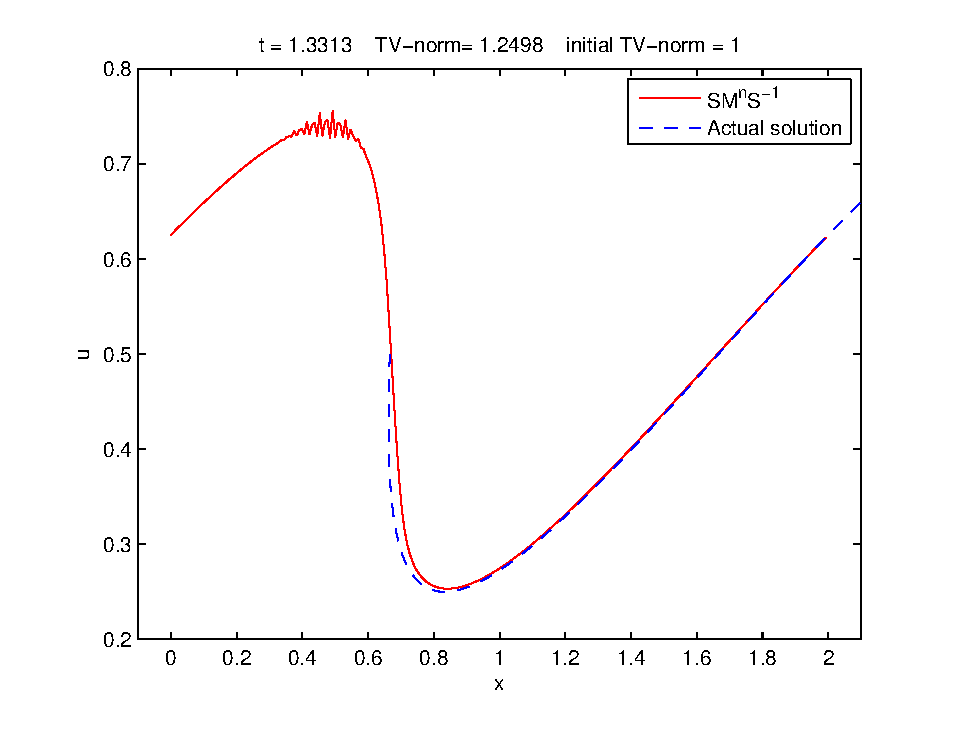
\includegraphics[width=0.45\textwidth]{Pictures/burgers_cont_no_tvd}}
    \caption{Solution of Burgers' equation with continuous initial data, using a 
    $TM^{n-2}R$ scheme, where $ M $ is ESSPRK($10,4,2$). 
    The SSP coefficient is $\sspcoef = 6.0$. 
    Here $TV$ denotes the difference between the $TV$-norms of the final and 
    initial solution.
    A positive sign indicates a violation of the TVD condition.}
    \label{fig:burgers_cont}
\end{figure}
%\yiannistodo{Elaborate more: Sharpness of SSP coefficient} 
%We were able to determine when exactly the nonlinear stability is not 
%satisfied by computing the the total-variation (TV) norm at each step of the 
%computation process. 
%This indicates that the ESSPRK-scheme inherits the time-step restriction 
%from the SSP coefficient of the main method $M$.
We measure these oscillations by computing the total variation.
It turns out that \textbf{\red TODO $\sigma = x.yz$}
is the largest value of $\sigma$ for which the total variation has not
increased at the final time.
This is \textbf{\red TODO $xy\%$} larger the value SSP coefficient
$\sspcoef = 6$.
\colintodo{In the figures, I would prefer to just report the TV
  itself, instead of this TV error.}


We also consider Burgers' equation with a discontinuous
square wave initial condition
\begin{equation*}%\label{eq:burgers_discont_IC}
    U(0,x)  = \left\{
                \begin{array}{ll}
                  1, & \hbox{$0.5 \leq x \leq 1.5$} \\
                  0, & \hbox{otherwise.}
                \end{array}
              \right.
\end{equation*}
Figure~\ref{fig:burgers_discont} shows the result of solving the 
discontinuous problem using an ESSPRK-scheme, where $M$ is an 
SSPRK($10,4,2$) method.
\begin{figure}
    \centering
    \subfloat[$\sigma = 6.0$]{\label{fig:burgers_discont_a}
      \includegraphics[width=0.45\textwidth]{Pictures/burgers_discont_tvd.eps}}
    \quad
    \subfloat[$\sigma = 6.18$]{\label{fig:burgers_discont_b}
      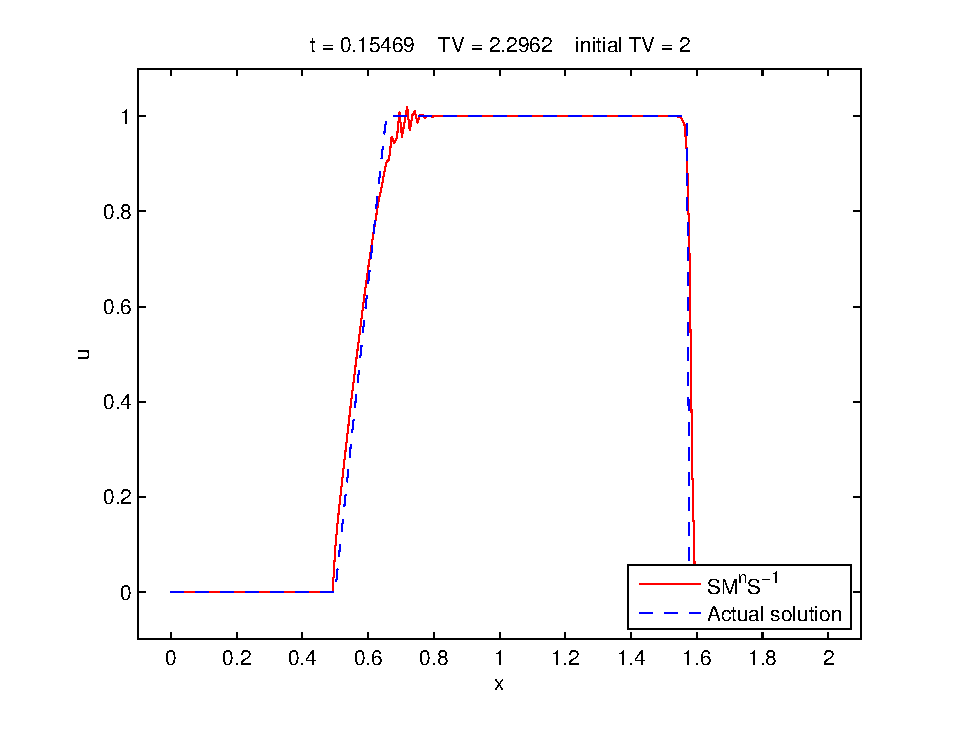
\includegraphics[width=0.45\textwidth]{Pictures/burgers_discont_no_tvd.eps}}
    \caption{Solution of Burgers' equation with discontinuous initial data, using a 
    $TM^{n-2}R$ scheme, where $M$ is SSPRK($10,4,2$) method. 
    The SSP coefficient is $ \sspcoef = 6.0$.
    Here $TV$ denotes the difference between the $TV$-norms of the final and 
    initial solution.
    A positive sign indicates a violation of the TVD condition.}
    \label{fig:burgers_discont}
\end{figure}
In this case, \textbf{\red TODO $\sigma = x.yz$} appears to be the
largest value of $\sigma$ for which the total variation has not
increased at the final time.
This is \textbf{\red TODO $xy\%$} larger than the SSP coefficient
$\sspcoef = 6$.

It is interesting to note that the stability prediction of the SSP
coefficient for ESSPRK is quite tight compared to other SSP methods
(c.f., \cite[Table 5.1]{Ketcheson/Gottlieb/Macdonald:TSRK}).
This may make effective order methods an interesting test case for
further research into both SSP time-discretizations as well as spatial
discretizations with strong stability features.


We also note the necessity of our $RM^{n-2}T$ approach: in this
example if we were to use the original approach of $S$ and $S^{-1}$,
the solution exhibits oscillations immediately following the
application of the starting perturbation scheme $S$.
%This is illustrated in Figure~\ref{fig:burgers_starting_method}


% The ESSPRK-scheme preserves monotonicity in the TV-norm since the starting 
% method $R$ is SSP.
% Using the original approach with $S$ and $S^{-1}$, the results are not
% SSP and the total-variation increases after the perturbation $S$.
% This is illustrated in Figure~\ref{fig:burgers_starting_method} in which 
% the solution is plotted after one application of methods $R$ and $S$ as the 
% starting procedures.
% % Note: its not really a step for %S% so I said application
% \begin{figure}
%     \centering
% 	TODO
% 	\yianniscomment{This should be cut out since if we optimize directly for R and T, we are not mentioning S.}
%     \caption{Solution of Burgers' equation with discontinuous initial data 
%     after one step, using a $TM^{n-2}R$ scheme, where $M$ is an 
%     SSPRK($5,4,2$) method. The solution is advanced one step by using (a) $R$ and 
%     (b) $S$}
%     \label{fig:burgers_starting_method}
% \end{figure}


        \section{Conclusion}\label{sec:Conclusion}
The theory of strong-stability preserving time discretization has been 
combined with the algebraic interpretation of effective order Runge--Kutta 
methods. 
Based on this concept, we succeeded in constructing the first explicit 
effective order SSP Runge--Kutta (ESSPRK) methods. 
These methods when accompanied with relative staring and finishing 
procedures result to schemes that attain higher order than the order of 
the constructing methods. 
It is proved that explicit Runge--Kutta methods with strictly positive 
weights have at most fourth effective order. 
This generates a barrier for explicit effective order SSP methods and 
hence we studied ESSPRK methods of third and fourth effective order.

Optimal ESSPRK methods were constructed and we studied their SSP 
properties in comparison with the classical SSPRK methods for linear and 
nonlinear problems. 
We were able to find families of third effective order ESSPRK methods. 
Also, despite the non existence of four-stage, four-order SSPRK methods, 
we found fourth effective order methods with four stages and of classical 
order two and three. 

Going beyond the initial formulation of the effective order schemes, a 
different choice of the starting and finishing methods allows the 
formation of an overall SSP scheme. 
The starting method not only perturbs but also advances the solution by 
a single time-step.  
Then the main ESSPRK method carries out the rest of the computation. 
At the final step a correction is applied by using a finishing method which 
basically eradicates the accumulated effect of the starting method. 
As a result the numerical approximation has order of accuracy equal to 
the effective order of the main method and thus higher than its classical 
order. 
The starting and finishing methods have minimal computation cost as 
they contain at most two more stages than those of the main method.

Finally, we performed numerical tests on nonlinear problems. In this way 
we showed that the schemes achieved their desired order. 
Moreover, we emphasized the importance of the SSP coefficient as an 
indicator of the maximum possible time-step for the solution of 
hyperbolic pdes. 
As shown in the case of Burgers' equation allowing slightly bigger time-steps 
than the theoretical bounds results in a highly oscillatory numerical 
approximation.  

\subsection{Future Work}\label{subsec:future_work}
The ideas here were applied to explicit Runge--Kutta methods, but they
can be applied to implicit Runge--Kutta methods and General Linear
Methods \cite{Butcher2008_book}.

Also, other possible directions may be the investigation of low-storage 
effective order SSP methods and advancing the SSP theory of effective 
methods. 
Finally, application of the effective order theory on other classes of 
methods, for example Rosenbrock methods, is also worthy of future 
research.

        \section*{Acknowledgments}{%
                The authors would like to thank the anonymous referees for their helpful 
                and valuable suggestions on the paper.
                \vspace*{20pt}
         }%
		
        %%% Appendix and Bibliography %%%
        %\appendix
        %% appendix A
\section{Proofs}\label{appendixA}

%\subsection{Proof of Theorem~\ref{thm:positiveb}}


	          
        \bibliographystyle{acm} % other style: apalike
        %\bibliographystyle{siam}  % turn on for siam style
        \bibliography{bibliography2}
		
\end{document}
